We now investigate three aspects of the results of this work.
First, we compare the output from the model to real-world data, on a qualitative level.
We then discuss the region of parameter space for which the model produces aphysical results.
Finally, we draw connections between chimera states in the model and their physiological analogues.
\subsection{Model Quality}
\label{sec:results_model}
The model used for this work was the modified Hindmarsh-Rose neural model\footnote{The modification is to add in the coupling, turning it into a network model instead of a single neuron.} \cite{Santos2017}.
\begin{align}
  \label{eq:hr_x}
  \dot{\hrx}_{j}
  &=
    \hry_{j}
    -
    \hrx_{j}^{3}
    +
    b \hrx_{j}^{2}
    +
    I_{j}
    -
    \hrz_{j}
    -
    \frac{\hra}{n'_{j}} \sum_{k = 1}^{N} G'_{j k} \Theta_{j}(\hrx_{k})
    -
    \frac{\hrb}{n''_{j}} \sum_{k = 1}^{N} G''_{j k} \Theta_{j}(\hrx_{k}) \\
  \label{eq:hr_y}
  \dot{\hry}_{j}
  &=
    1
    -
    5 \hrx_{j}^{2}
    -
    \hry_{j} \\
  \label{eq:hr_z}
  \dot{\hrz}_{j}
  &=
    \mu \pqty{s \pqty{\hrx_{j} - \hrx_{\text{rest}}} - \hrz_{j}}
\end{align}
where
\begin{equation}
  \label{eq:hr_sigmoid}
  \Theta_{j}(\hrx_{k})
  =
  \frac{\hrx_{j} - \hrx_{\text{rev}}}{1 + e^{-\lambda \pqty{\hrx_{k} - \theta}}}
\end{equation}
is the sigmoidal activation function, making it a neural mass model.
\Cref{tab:hr_params} shows the values and meanings of the symbols in the model.

\begin{table}[ht]
  \centering
  \begin{tabular}{c | c | l}
    Symbol & Value & Meaning \\ \hline
    $\hrx_{j}$ & --- & Membrane potential of the $j$th neural mass \\
    $\hry_{j}$ & --- & Associated with the fast processes \\
    $\hrz_{j}$ & --- & Associated with slow processes \\ \hline
    $b$ & 3.2 & Tunes the spiking frequency \\
    $I_{j}$ & 4.4 & External input current \\
    $\hrx_{\text{rev}}$ & 2 & Ambient reverse potential \\
    $\lambda$ & 10 & Sigmoidal activation function parameter \\
    $\theta$ & -0.25 & Sigmoidal activation function parameter \\
    $\mu$ & 0.01 & Time scale for variation of $z$ \\
    $s$ & 4 & Governs adaptation \\
    $\hrx_{\text{rest}}$ & -1.6 & Resting/equilibrium potential \\ \hline
    $\hra$ & Varied & Connection strength within cortices \\
    $n_{j}'$ & See \cref{fig:n_prime} & Number of connections within a cortex from the $j$th neuron \\
    $G_{j k}'$ & See \cref{fig:g_prime} & Intra-cortical connection matrix \\
    $\hrb$ & Varied & Connection strength between conrtices \\
    $n_{j}''$ & See \cref{fig:n_prime} & Number of connections between cortices from the $j$th neuron \\
    $G_{j k}''$ & See \cref{fig:g_prime} & Inter-cortical connection matrix
  \end{tabular}
  \caption[Hindmarsh-Rose Parameters]{The list of parameters used in modeling the Hindmarsh-Rose network.}
  \label{tab:hr_params}
\end{table}

This model was chosen due to the semanticity of its parameters, as well as its proven ability to exhibit chimera-like behavior as a neural mass model \cite{Santos2017}.
Additionally, the Hindmarsh-Rose model was not designed to emulate seizures, which provides further evidence for the theory that chimeras are a universal aspect of brain activity, as discussed in \cref{sec:lit_review_chimera_square_torus}.

%%% Local Variables:
%%% mode: latex
%%% TeX-master: "../../main"
%%% End:


\subsection{Aphysical Region}
\label{sec:results_aphysical}
We choose not to include figures for the first two sweeps of \cref{tab:parameter_sweeps} because a large portion of parameter space leads to an aphysical model.
Specifically, for certain value pairs of $\pqty{\hra, \hrb}$, certain neurons never fired (increased past 1).
Despite the drastically increased time of evaluation (see \cref{sec:methods_implementation}), a vast swath of parameter space gave nonsense results (the white shown in \cref{fig:aphysical_chimera}).
\begin{figure}[ht]
  \centering
  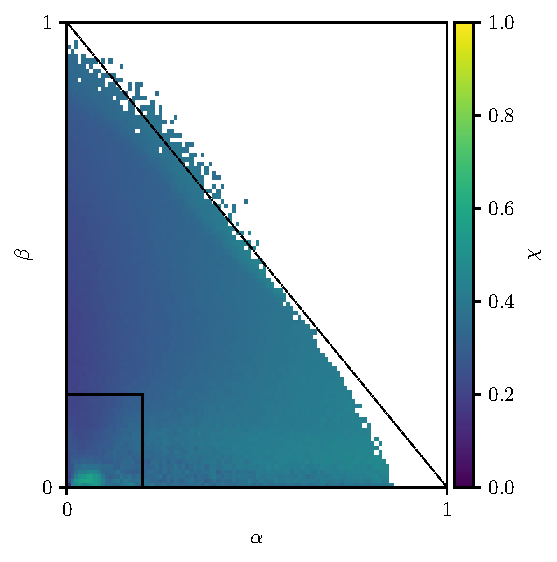
\includegraphics[width=\columnwidth]{figure/aphysical_chimera_100dpi.pdf}
  \caption[Chimera-like index landscape]{
    The chimera-like landscape of parameter space on $\pqty{\hra, \hrb} \in \pqty{0, 1.0} \times \pqty{0, 1.0}$.
    The aphysical region of the model is shown in white.
    The black rectangle in the bottom left corner indicates the region of parameter space shown in \cref{fig:zoom}.
    The dashed line has a slope of $-1$, to serve as a guide for \cref{sec:results_chimera}.
    The chimera-like index (defined in \cref{eq:chimera}) is normalized to $\frac{1}{7}$, as usual.
  }
  \label{fig:aphysical_chimera}
\end{figure}
The boundary between physical and aphysical appears to be linear, with a negative slope.
This means that $\hra$ can range further when $\hrb$ is low,
and vice versa.
This makes sense, as increased $\hra$ and $\hrb$ influence the model in the same way (increasing the coupling and decreasing $\dot{\hrx}_{j}$).

Furthermore, the slope of the boundary is greater than $-1$, which means that $\hra$ has an greater influence on the physicality of the model.
This is also reasonable, but for slightly less self-evident reasons.
To explain why, we must look specifically at the coupling term from \cref{eq:hr_x}:
\[
  -\frac{\hra}{n'_{j}} \sum_{k = 1}^{N} G'_{j k} \Theta_{j}\pqty{\hrx_{k}}
  -
  \frac{\hrb}{n''_{j}} \sum_{k = 1}^{N} G''_{j k} \Theta_{j}\pqty{\hrx_{k}}.
\]
This coupling will, in fact, be positive, as $\Theta_{j}\pqty{\hrx_{k}} < 0$ if $\hrx_{j} < 2$, which is true almost all of the time.
This means that, as $\hra$ and $\hrb$ increase, so does the overall coupling strength.
So, there is some threshold $K$ for which the overall coupling is too strong if, for some $j$,
\begin{equation}
  \label{eq:coupling_inequality}
  \frac{\hra}{n'_{j}} \sum_{k = 1}^{N} G'_{j k} \abs{\Theta_{j}\pqty{\hrx_{k}}}
  +
  \frac{\hrb}{n''_{j}} \sum_{k = 1}^{N} G''_{j k} \abs{\Theta_{j}\pqty{\hrx_{k}}}
  >
  K_{j}.
\end{equation}
In order for $\hra$ to influence the coupling's proximity to $K$ more than $\hrb$ does, there must exist some $j$ such that
$\frac{1}{n'_{j}} \sum G'_{j k} \abs{\Theta_{j}\pqty{\hrx_{k}}}
>
\frac{1}{n''_{j}} \sum G''_{j k} \abs{\Theta_{j}\pqty{\hrx_{k}}}$.
Seeing as $\overline{g}'_{j} = \frac{1}{n'_{j}} \sum G'_{j k}$ and $\overline{g}''_{j} = \frac{1}{n''_{j}} \sum G''_{j k}$ are the average connection strength within and between cortices (shown in \cref{fig:average_strengths} A), these are simply a function of the topology of the graph.

It may look from \cref{fig:average_strengths} A like $\hrb$ should have more influence than $\hra$, as for most $j$, $\overline{g}''_{j} > \overline{g}'_{j}$.
However, for most of those cases, $\overline{g}'_{j_{0}} > \overline{g}''_{j_{0}} = 0$.
This means that, for those $j_{0}$, $\pdv{K_{j_{0}}}{\hra} = 0$.
So, those cases contribute to the value of the threshold, but do not influence the physicality's dependence on $\hra$ and $\hrb$.

If we remove the $j$ for which $0 \in \Bqty{\overline{g}'_{j}, \overline{g}''_{j}}$, we find that, on average, $\overline{g}'_{j} = 2.100$, slightly more than $\overline{g}''_{j} = 2.079$ (see \cref{fig:average_strengths} B).
This explains the slope of the boundary between the physical region and the aphysical region.

%%% Local Variables:
%%% mode: latex
%%% TeX-master: "../../ms"
%%% End:


\subsection{Chimera states}
\label{sec:results_chimera}
We show the normalized chimera-like index of the entire physical region in \cref{fig:aphysical_chimera}.
Near the maximal edge of the physical region, the highest values of the chimera index appear to follow a slope of $-1$.
It is unsurprising that chimera states would be prevalent when the coupling is large (out near the boundary of the aphysical range).

What is surprising, however, is the presence of the chimeric patch in the bottom left corner of \cref{fig:aphysical_chimera}, shown at a higher resolution in \cref{fig:zoom}.
\begin{figure}[ht]
  \centering
  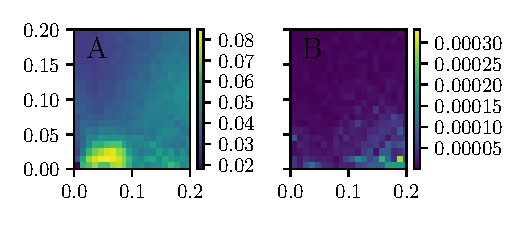
\includegraphics[width=0.5\textwidth]{figure/zoom_100dpi.pdf}
  \caption[Zoomed landscape]{A.\ The chimera-like index $\chimera$ of runs with $(\hra, \hrb) \in (0, 0.2) \times (0, 0.2)$.
    As before, the chimera-like index is normalized to $\frac{1}{7}$.
    Note that the values of the index are much higher in this patch than in most of the rest of $(\hra, \hrb) \in (0, 1) \times (0, 1)$ (\cref{fig:aphysical_chimera}).
    B.\ The variance of the chimera-like index.
  }
  \label{fig:zoom}
\end{figure}
Plotting the results of the simulations (\cref{fig:041_021}),
it is evident that this is not a calculation error, but is an actual feature of the parameter landscape.
\begin{figure*}[ht]
  \centering
  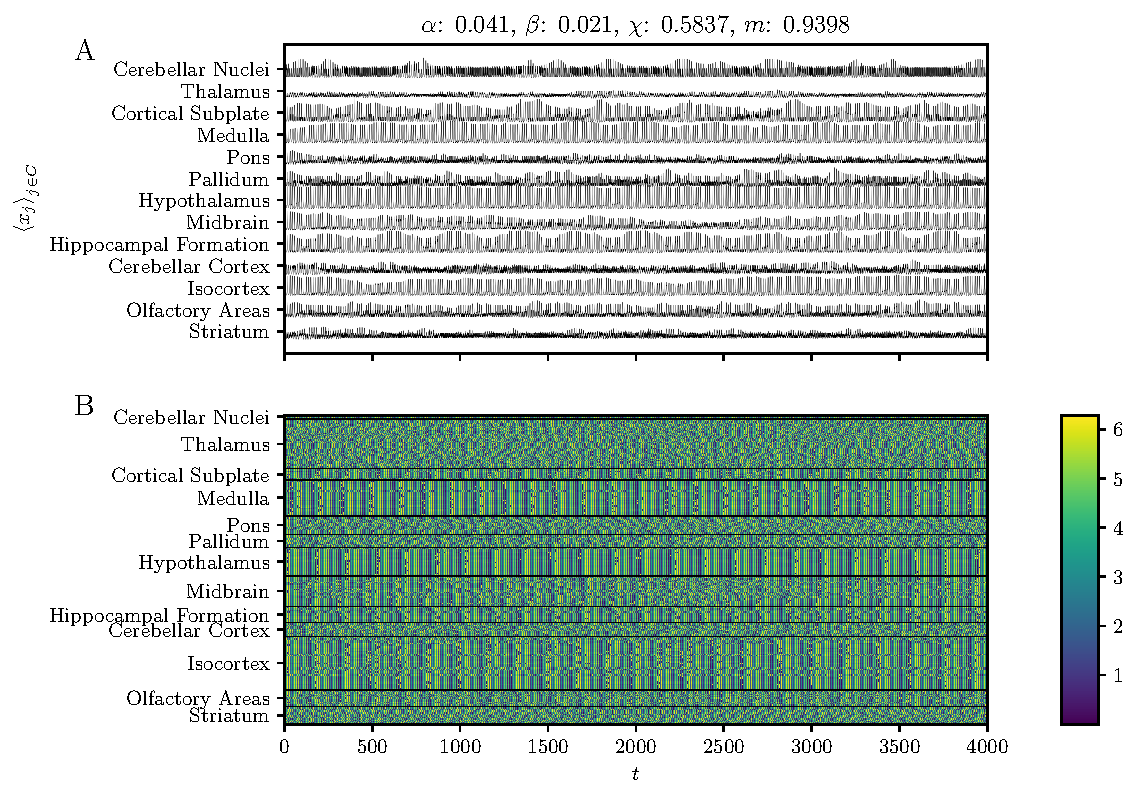
\includegraphics[width=\textwidth]{figure/0_041-0_021_200dpi.pdf}
  \caption[Highly chimeric simulation]{A run of the Hindmarsh-Rose simulation in the chimeric island.
    A. The mean membrane potential within each cortex.
    B. The phase $\phase$ of the entire timeseries for a simulation of the Hindmarsh-Rose network.
    Synchronization is most consistently evident in the medulla, the hypothalamus, and the isocortex.
  }
  \label{fig:041_021}
\end{figure*}

The highly chimeric patch within the physical portion of the landscape appears to be mostly below the $\beta = \alpha$ line.
This is reasonable, as chimera states occur when coupling within groups is greater than coupling between groups.
A small portion of the chimeric patch lies above the $\beta = \alpha$ line, likely because the average strength between cortices is greater than the average strength within cortices (see \cref{fig:average_strengths} A).

The chimera-like index $\chimera$ greatly lessens at $\alpha \approx 0.1$.
A possible explanation for this comes from comparing the order of $\dot{\hrx}$ without the coupling terms, and the coupling terms themselves.
From our simulation, we find that $\dot{\hrx}$ without the coupling terms ranges roughly from -6 to 3.
The coupling terms each\footnote{Since the same can be said for both $\alpha$ and $\beta$, we will discuss only $\alpha$, with the understanding that $\beta$ could be substituted into the proceeding sentences.}
range from 0 to approximately $30 \alpha$.
This means that, when $\alpha > 0.1$, the coupling is at least of the same order as the sum of the rest of the terms in the equation.
This leads to a qualitative difference between the two states, which likely manifests itself as the less-chimeric states.

%%% Local Variables:
%%% mode: latex
%%% TeX-master: "../../ms"
%%% End:

